\section{Gates} \label{sec:gates}

Each gate is a row with 135 columns. As different custom gate has different complexity, for some complex gate 135 columns may only constraints one
operation while for other simple gate 135 columns may constraints several operations. The index of operation in a row is called slot.

Steps to use a custom gate:
\begin{itemize}
    \item Determine the type of gate;
    \item Find row and slot using gate type;
    \item Wire the operation parameters to cells found;
\end{itemize}

For the convenience of description, the trace tables in this paper only show one operation which is slot is 0.

\subsection{Custom gates}
\subsubsection{arithmetic\_base}

ArithmeticGate is a gate which can perform a weighted multiply-add, i.e.
\[ \text{res} = \text{cons\_0} \times \text{mul\_0} \times \text{mul\_1} + \text{cons\_1} \times \text{add}. \]

The structure of gate is shown in \figref{fig:arithmetic-gate}.

\begin{figure}[!ht]
    \centering
    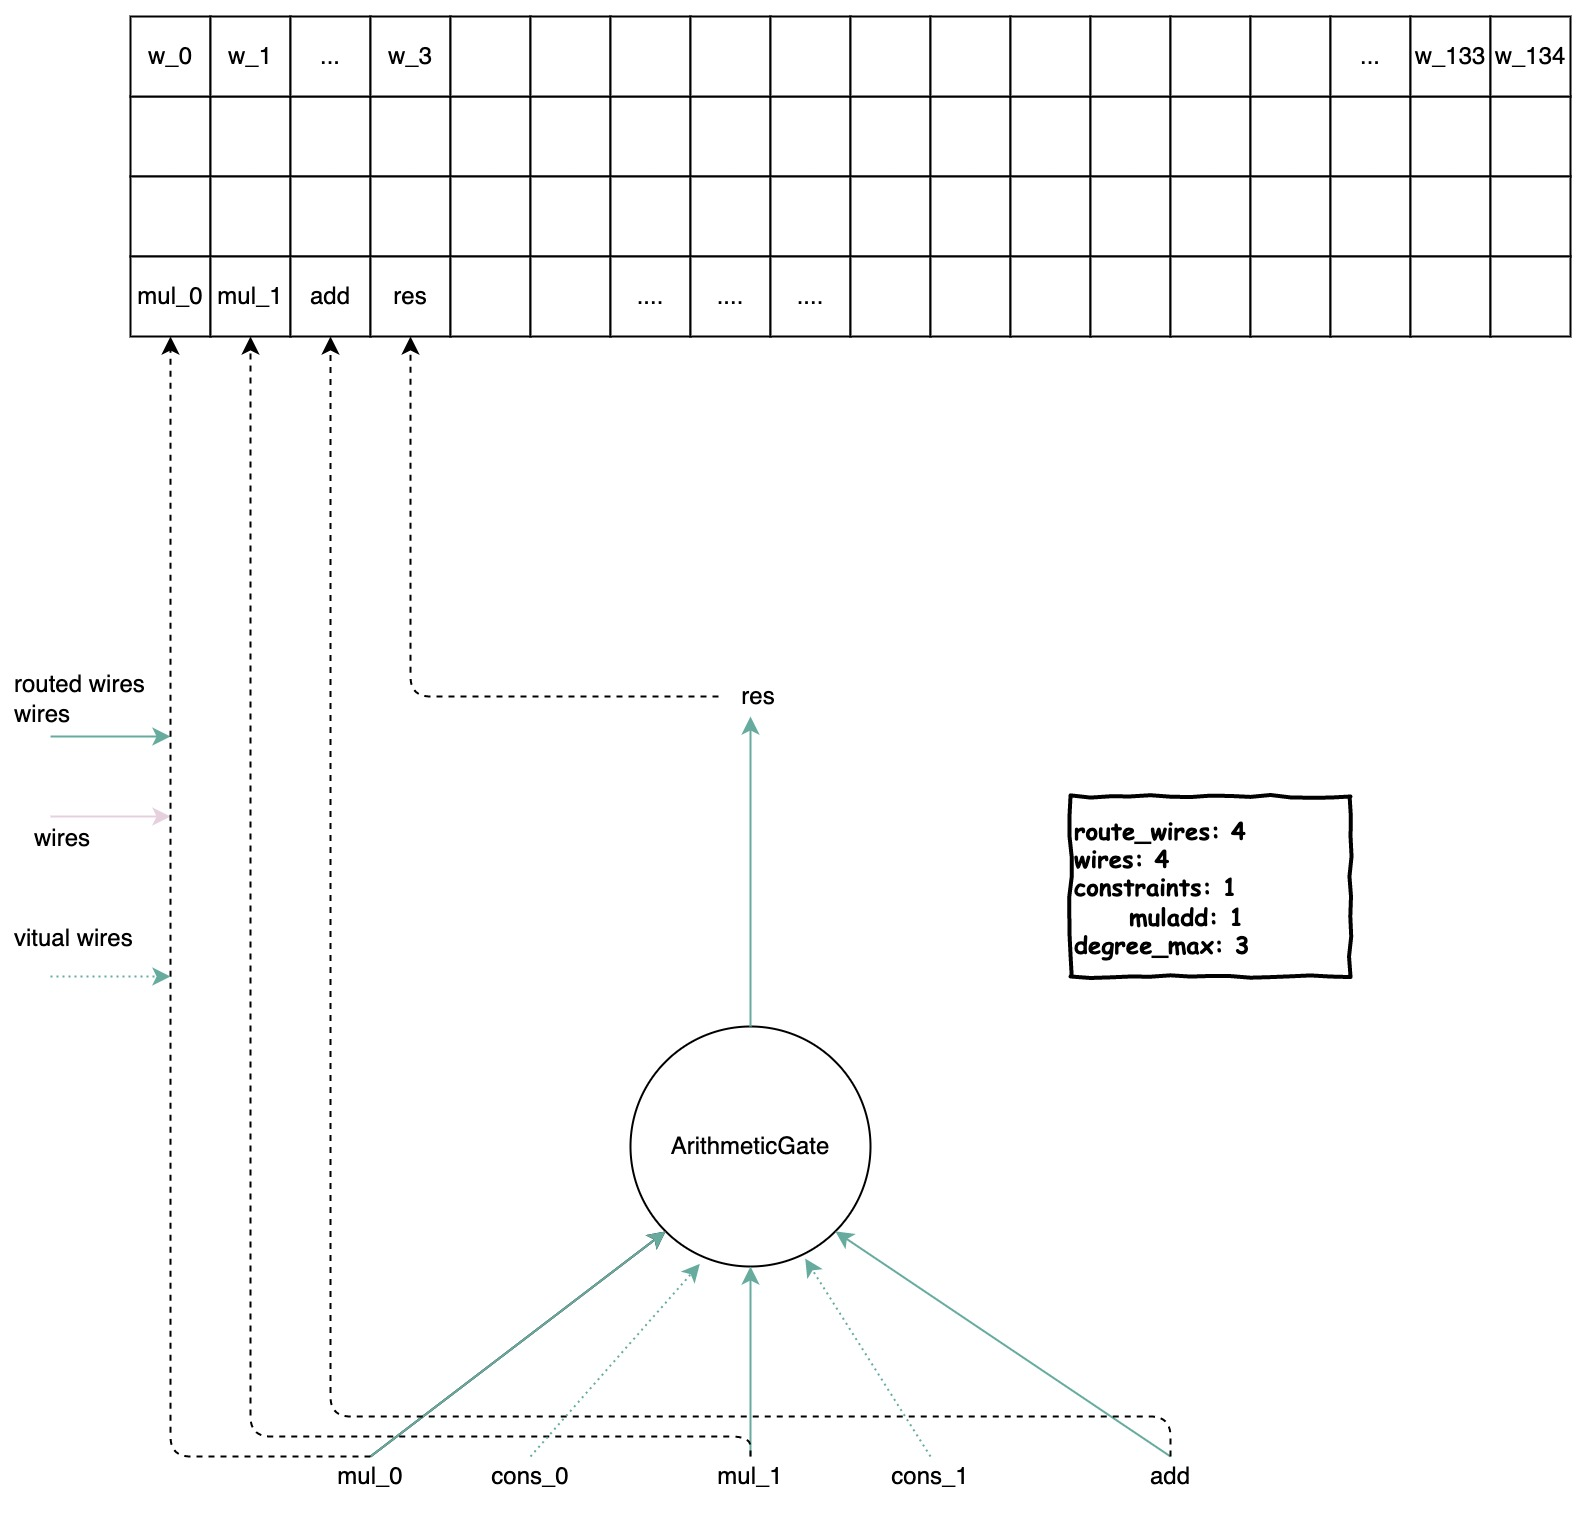
\includegraphics[width=0.8\textwidth]{gates/arithmetic_base.jpeg}
    \caption{ArithmeticGate}
    \label{fig:arithmetic-gate}
\end{figure}

There's only one constraint per operation, and degree is 3.

\subsection{arithmetic\_extension}

To understand the design principle of this Gate, we must first understand \href{https://en.wikipedia.org/wiki/Field_extension#Extension_field}{Field extension}. 


Taking Plonky2's GoldilocksField as an example, we give the extension field elements under quadratic, quadratic and quintuple expansions respectively:

\begin{figure}[!ht]
    \centering
    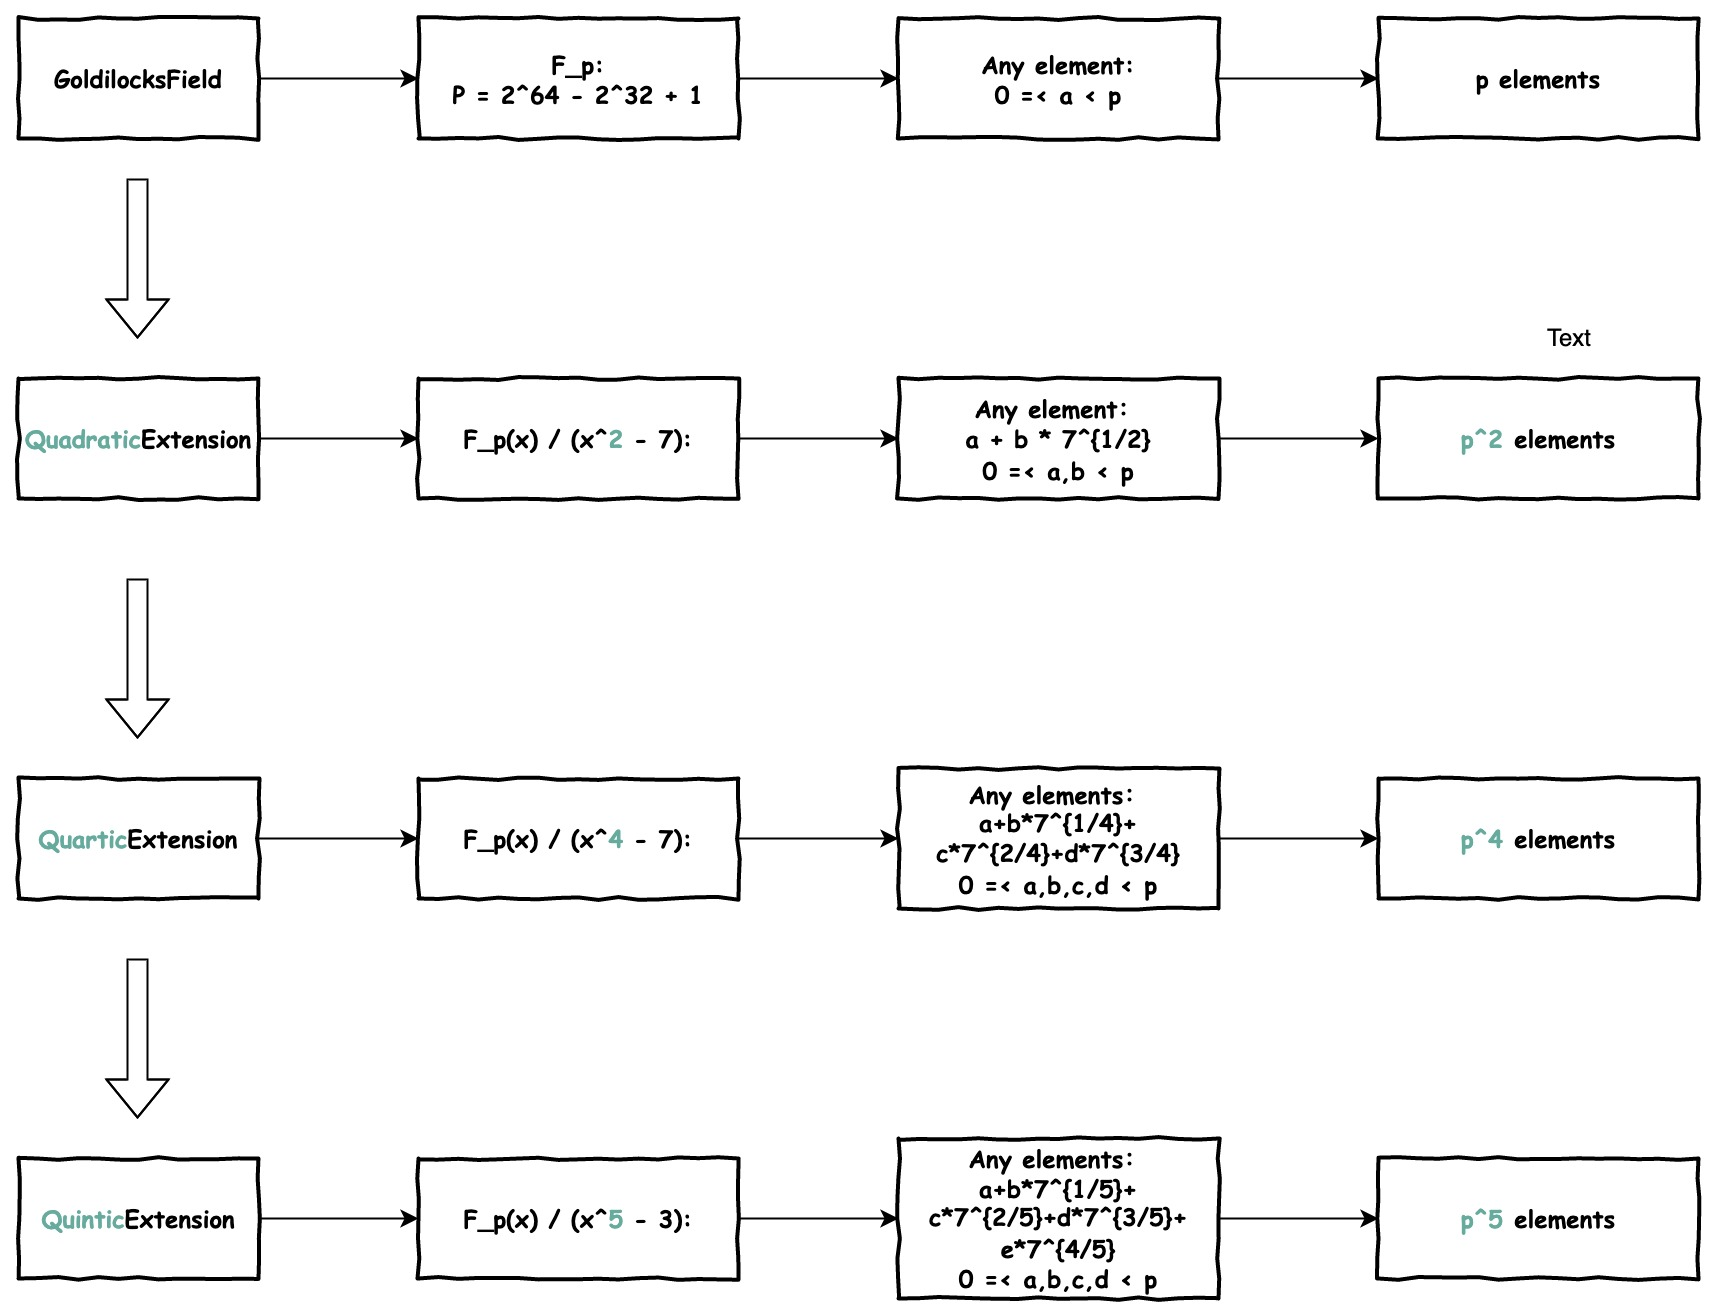
\includegraphics[width=0.8\textwidth]{gates/arthmetic_extension_ext.jpeg}
    \caption{GoldilocksField Extension}
    \label{fig:goldilocksfield-extension}
\end{figure}

It is easy to see that for QuadraticExtension Field, the elements on its domain take the form $a + b \sqrt{7}; a,b \subset F_p$, and a, b cannot both be 0.
It can be seen that on the quadratic extension domain, there are $p^2$ elements and the original domain is a subset of the quadratic extension domain.

ArithmeticExtensionGate is also a gate which can perform a weighted multiply-add, i.e.
\[res = cons\_0 * mul\_0 * mul\_1 + cons\_1 * add\]
The elements of the QuadraticExtension Field are represented in the form $[a, b]$, so the Gate design for arithmetic\_extension has the following form:

\begin{figure}[!ht]
    \centering
    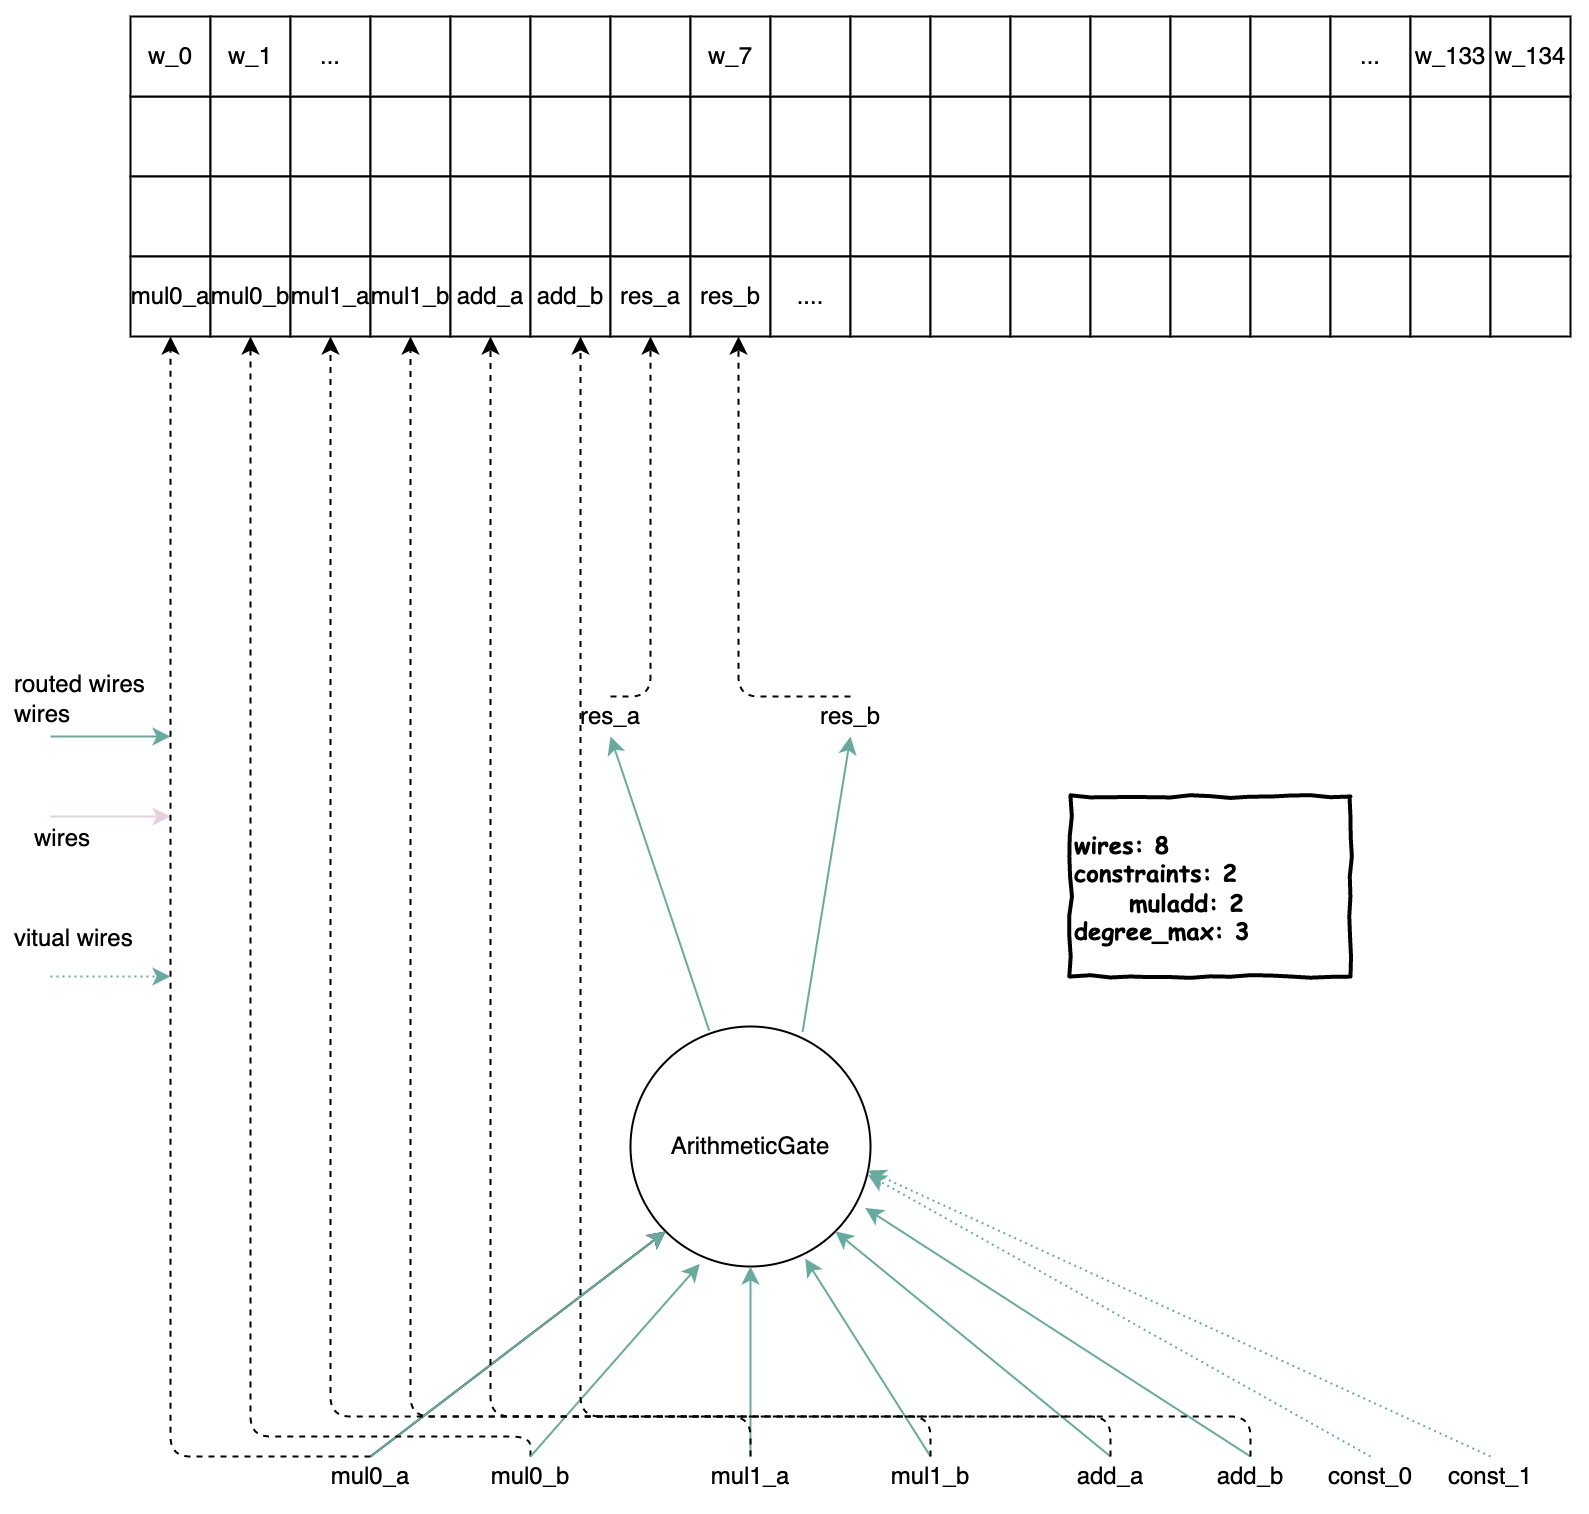
\includegraphics[width=0.8\textwidth]{gates/arthmetic_extension.jpeg}
    \caption{ArithmeticExtensionGate}
    \label{fig:arthmetic-extension}
\end{figure}
\subsubsection{base\_sum}

BaseSumGate is used to constrain the input to be composed of limbs which are arranged in little-endian. There are two kinds of constraints:

For each limb, limb is in range [0, base):
\[\sum_{i=0}^{base}(limb_i - i) = 0\]

Input is composed of limbs:
\[input = \sum_{i=0}^{n-1} limb_{n-1-i} * base^i\]

\begin{figure}[!ht]
    \centering
    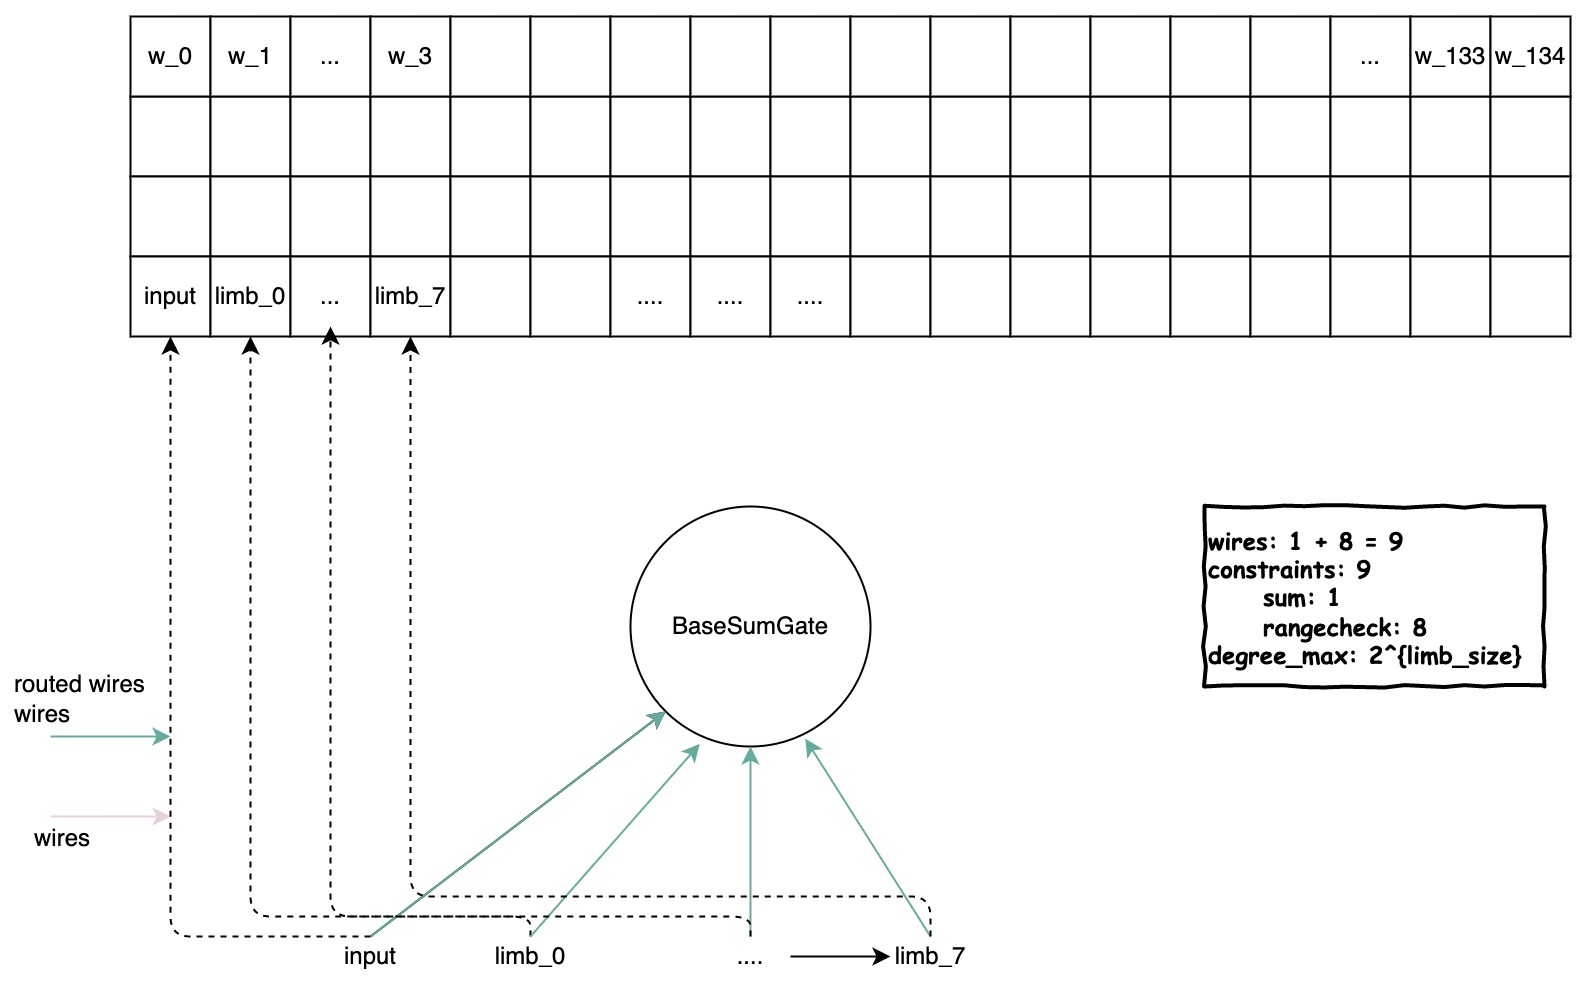
\includegraphics[width=0.8\textwidth]{gates/base_sum.jpeg}
    \caption{BaseSumGate}
    \label{fig:base-sum}
\end{figure}
\subsection{exponentiation}

ExponentiationGate is a gate for raising a value to a power. Trace table contains base, bits of the exponent, output, and intermediate value of the bits.

Take $A^{21} = A^{10101_b}$ for example to describe intermediate value, the bits are [1, 0, 1, 0, 1].

\begin{enumerate}
    \item Current bit=1, we start from 1, and times $A^{bit}$ we get $A$
    \item Current bit=0
    \begin{itemize}
        \item Square prev\_intermediate\_value $A^{1_b << 1} = A^{10_b}$
        \item Then times $A^{bit}$ we get $A^{10_b} * A^0 = A^{10_b}$
    \end{itemize}
    \item Current bit=1
    \begin{itemize}
        \item Square prev\_intermediate\_value $A^{10_b<<1} = A^{100_b}$
        \item Then times $A^{bit}$ we get $A^{100_b} * A = A^{101_b}$
    \end{itemize}
    \item Current bit=0
    \begin{itemize}
        \item Square prev\_intermediate\_value $A^{101_b << 1} = A^{1010_b}$
        \item Then times $A^{bit}$ we get $A^{1010_b} * 1 = A^{1010_b}$
    \end{itemize}
    \item Current bit=1
    \begin{itemize}
        \item Square prev\_intermediate\_value $A^{1010_b << 1} = A^{10100_b}$
        \item Then times $A^{bit}$ we get $A^{10100_b} * A = A^{10101_b}$
    \end{itemize}
\end{enumerate}

And we get the last intermediate value $A^{10101_b}$ which should be equal to the output.

Let's take another example of a specific number $2^13 = 2^{1101_b}$, and have a look at the trace cell:
\begin{center}
    \begin{tabular}{ |c|c|c|c|c|c|c|c|c|c| }
        \hline
        base & b\_0 & b\_1 & b\_2 & b\_3 & output & inter\_0 & inter\_1 & inter\_2 & inter\_3 \\
        \hline
        2 & 1 & 0 & 1 & 1 & 8192 & 2 & 8 & 64 & 8192 \\
        \hline
    \end{tabular}
\end{center}

The structure of Gate is shown in the figure:
\begin{figure}[!h]
    \centering
    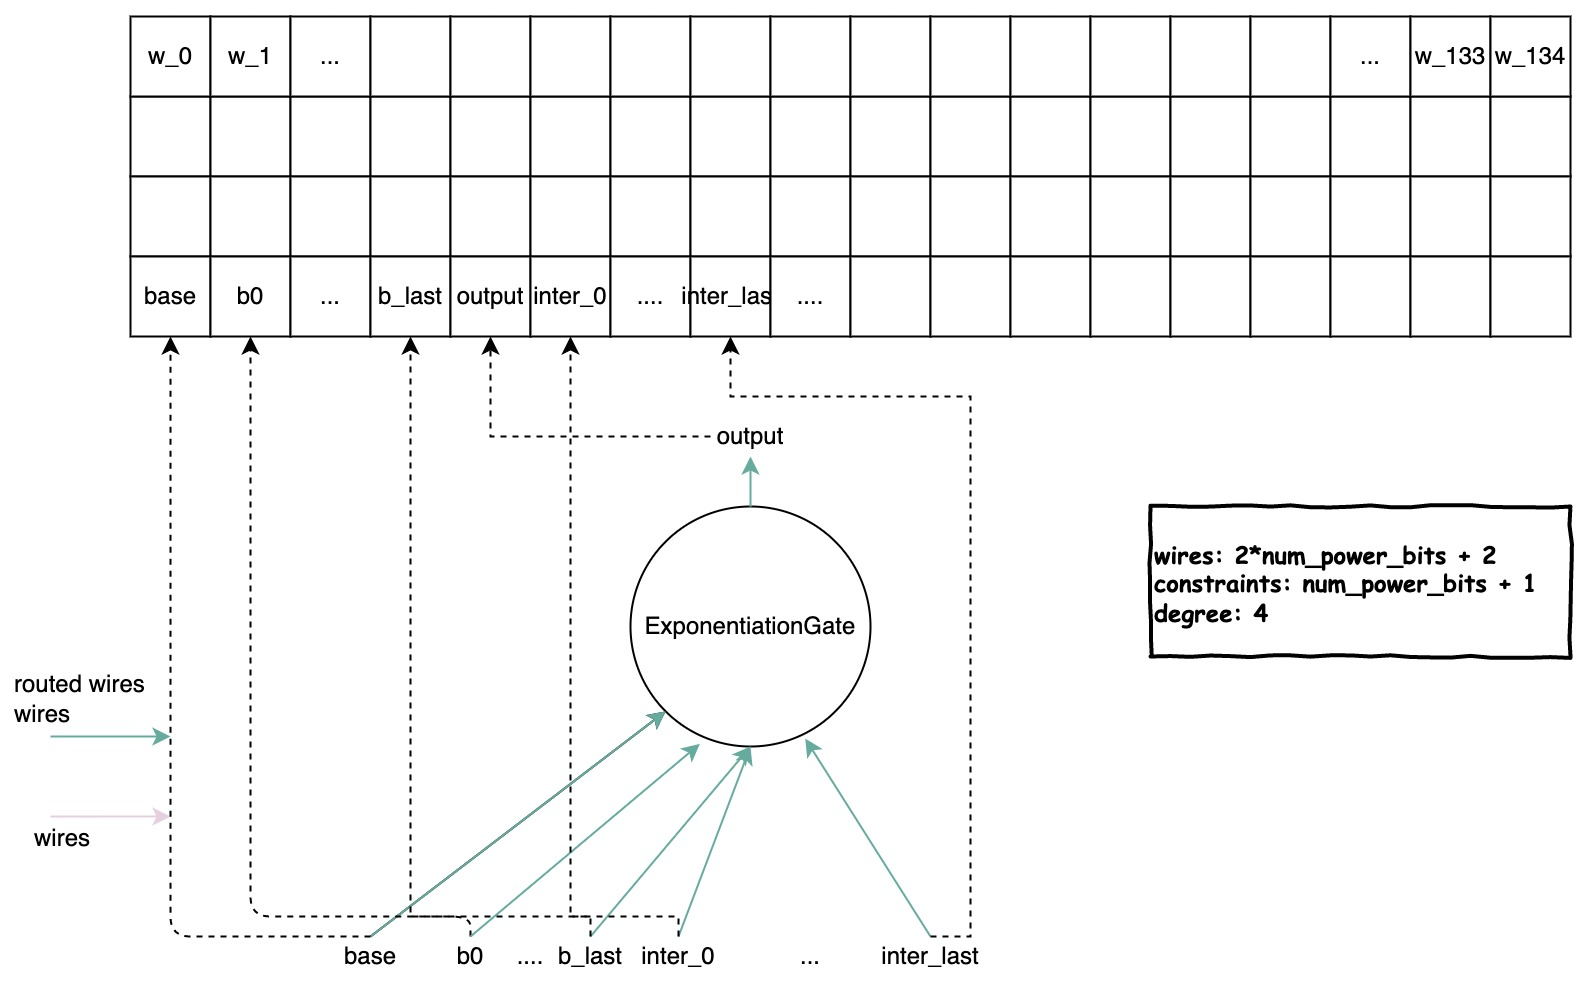
\includegraphics[width=0.8\textwidth]{gates/exponentiation.jpeg}
    \caption{ExponentiationGate}
    \label{fig:exponetiation-gate}
\end{figure}
\subsection{poseidon}

\href{https://www.poseidon-hash.info/}{Poseidon} is a hash function designed for zero-Knowledge proof system.
Its calculation process is roughly as follows:

\begin{figure}[!h]
    \centering
    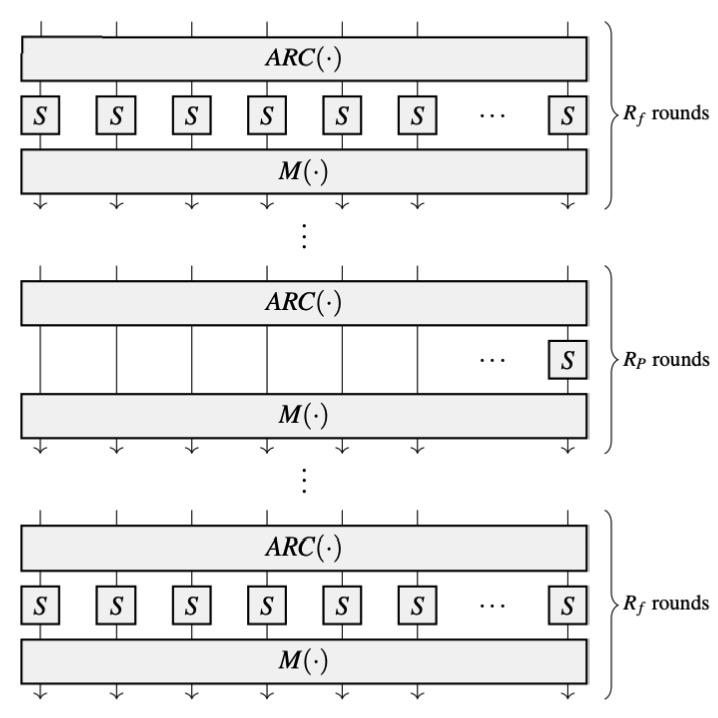
\includegraphics[width=0.8\textwidth]{gates/poseidon_process.jpeg}
    \caption{Construction of poseidon}
    \label{fig:poseidon-process}
\end{figure}

Each round function of poseidon permutation consists of the following three compoments.
\begin{enumerate}
    \item ARC(.): AddRoundConstants
    \item S: SubWords
    \item M(.): MixLayer
\end{enumerate}

Trace of the gate is like:
\begin{figure}[!h]
    \centering
    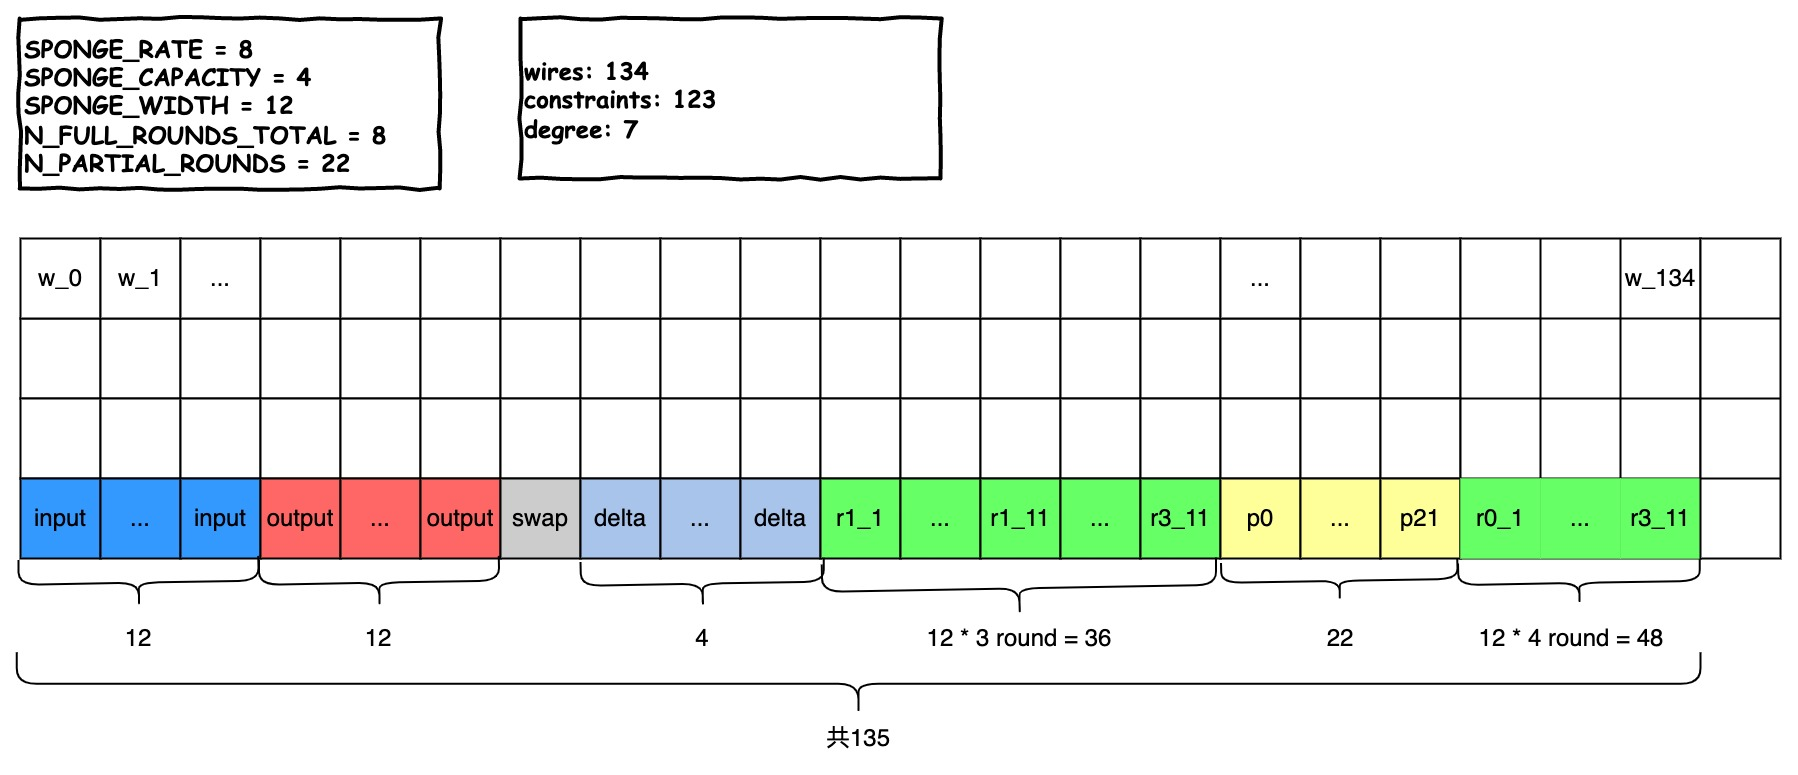
\includegraphics[width=0.8\textwidth]{gates/poseidon.jpeg}
    \caption{PoseidonGate}
    \label{fig:poseidon-gate}
\end{figure}

\begin{itemize}
    \item input: components of the input , 12 elements.
    \item output: components of the output, 12 elements.
    \item swap: 0 or 1, Indicates whether the first four elements of the input are swapped with the last four elements.
    \item delta: used when swap is 1, $delta_i = swap * (input_{rhs} - input_{lhs})$
    \item green region: full rounds, ri\_1~ri\_11 is the state of each round.
    \item yellow region: partial rounds, each element is state[0] of each round.
\end{itemize}

Calculation process and related constraints:
\begin{itemize}
    \item Assert that swap is binary. -- 1 constraint
    \begin{lstlisting}
constraints.push(swap * (swap - F::Extension::ONE))
    \end{lstlisting}
    \item Assert $delta_i = swap * (rhs - lhs)$ -- 4 constraints
    \begin{lstlisting}
for i in 0..4 {
    ....
    constraints.push(swap * (input_rhs - input_lhs) - delta_i);
}
    \end{lstlisting}
    \item Initialize state: when swap=0, state=input; when swap=1, state is swapped input:
    \begin{figure}[!h]
        \centering
        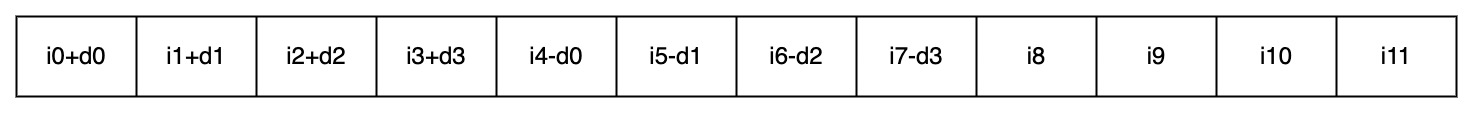
\includegraphics[width=0.8\textwidth]{gates/poseidon_state_init.jpeg}
        \caption{Poseidon State Init}
        \label{fig:poseidon-state-init}
    \end{figure}
    \begin{lstlisting}
for i in 0..4 {
    ...
    state[i] = vars.local_wires[input_lhs] + delta_i;
    state[i + 4] = vars.local_wires[input_rhs] - delta_i;
}
for i in 8..SPONGE_WIDTH {
    state[i] = vars.local_wires[Self::wire_input(i)];
}
    \end{lstlisting}
    \item Begin first full rounds calculation, for each round r(which is 0~3)
    \begin{itemize}
        \item Perform ARC: Add each element of state to the pre-generated value at a particular position in the array.
        \begin{lstlisting}
for i in 0..WIDTH {
    state[i] += F::from_canonical_u64(ALL_ROUND_CONSTANTS[i + WIDTH * round_ctr]);
}
        \end{lstlisting}
        \item Except for r=0, constrain each element of the state calculated in the previous round (the green part of the first slice of the figure). 
        -- 12 constraints per round, totally 36 constraints.
        \item Perform SubWords: Turn state element by element x into $x => x^7$
        \item Perform MixLayer: Each element of the state is updated according to itself and a pre-generated array.
        \begin{lstlisting}
// r is index of state elements here.
let mut res = F::ZERO;
    for i in 0..WIDTH {
    res += v[(i + r) % WIDTH] * F::from_canonical_u64(Self::MDS_MATRIX_CIRC[i]);
}
res += v[r] * F::from_canonical_u64(Self::MDS_MATRIX_DIAG[r]);
        \end{lstlisting}
    \end{itemize}
    \item Perform parial rounds:
    \begin{itemize}
        \item Perform ARC
        \begin{lstlisting}
for i in 0..12 {
    if i < WIDTH {
        state[i] += F::from_canonical_u64(Self::FAST_PARTIAL_FIRST_ROUND_CONSTANT[i]);
    }
}
        \end{lstlisting}
        \item Processing of state with MDS(maximum distance separable) matrix(11*11).
        \begin{lstlisting}
result[0] = state[0];
for r in 1..12 {
    if r < WIDTH {
        for c in 1..12 {
            if c < WIDTH {
                let t = F::from_canonical_u64(
                    Self::FAST_PARTIAL_ROUND_INITIAL_MATRIX[r - 1][c - 1],
                );
                result[c] += state[r] * t;
            }
        }
    }
}
result
        \end{lstlisting}
        \item Perform 22 round sbox, for the first 21 rounds (r = 0..=21):
        \begin{itemize}
            \item Take sbox\_in(yellow elements in the figure), and constrains state[0]=sbox\_in -- 21 rounds totally 21 constraints.
            \item $state[0]^=7$
            \item $state[0] += FAST\_PARTIAL\_ROUND\_CONSTANTS[r]$
            \item Perform mds to state.
        \end{itemize}
        \item For the 22th round:
        \begin{itemize}
            \item asdf
        \end{itemize}
    \end{itemize}
    \item Perform second round "Full rounds", same with the first round.(the green part of the second slice of the figure). -- 12 constraints, 4 rounds totally 48 constraints.
    \item Asserts computed result equals output. -- 12 constraints
    \begin{lstlisting}
for i in 0..SPONGE_WIDTH {
    constraints.push(state[i] - vars.local_wires[Self::wire_output(i)]);
}
    \end{lstlisting}
\end{itemize}
\subsubsection{poseidon\_mds}

This gate is used for constrain outputs of poseidon mds.

\begin{figure}[!h]
    \centering
    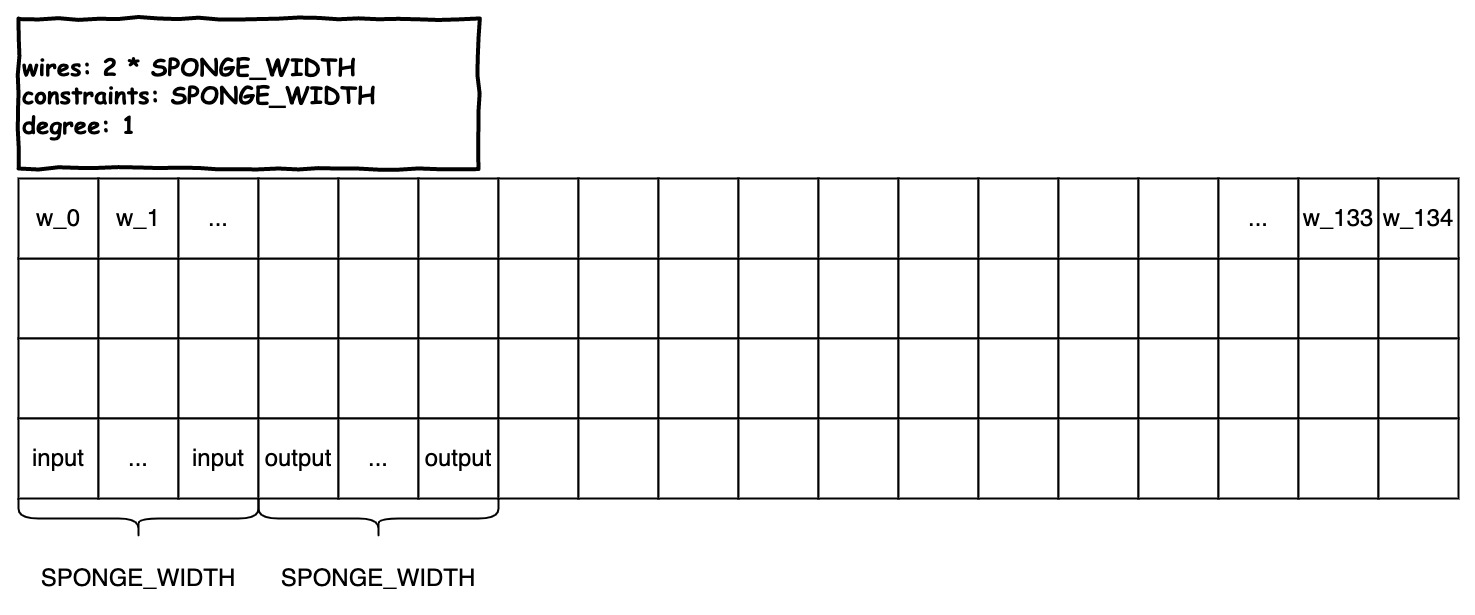
\includegraphics[width=0.8\textwidth]{gates/poseidon_mds.jpeg}
    \caption{PoseidonMdsGate}
    \label{fig:poseidon-mds}
\end{figure}

computed\_output is calculated from input, and constrained with output element by element, total 12 constraints(degree 1).
\begin{lstlisting}
let inputs: [_; SPONGE_WIDTH] = (0..SPONGE_WIDTH)
    .map(|i| vars.get_local_ext_algebra(Self::wires_input(i)))
    .collect::<Vec<_>>()
    .try_into()
    .unwrap();
let computed_outputs = Self::mds_layer_algebra(&inputs);
(0..SPONGE_WIDTH)
    .map(|i| vars.get_local_ext_algebra(Self::wires_output(i)))
    .zip(computed_outputs)
    .flat_map(|(out, computed_out)| (out - computed_out).to_basefield_array())
    .collect()
\end{lstlisting}
\subsubsection{random\_access}

RandomAccessGate is used for verify that an element matches a value in the list.

\begin{figure}[!ht]
    \centering
    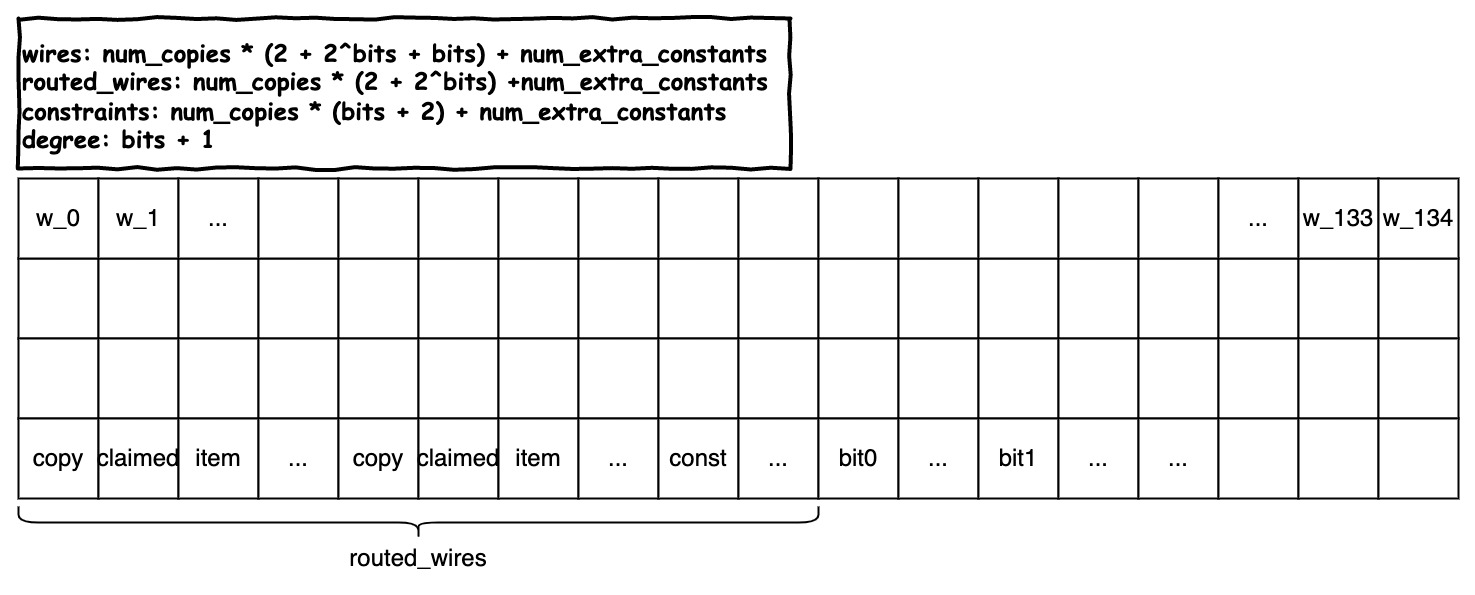
\includegraphics[width=0.8\textwidth]{gates/random_access.jpeg}
    \caption{RandomAccessGate}
    \label{fig:random-access}
\end{figure}

\begin{itemize}
    \item item: list items.
    \item copy: index of target element in the list
    \item claimed: target element
    \item bit\_i: bits for the i-th copy
\end{itemize}

For each copy:
\begin{itemize}
    \item Constrain bits are 0 or 1. -- bits constraints for each copy, A total of num\_copied*bits constraints.
    \begin{lstlisting}
for &b in &bits {
    constraints.push(builder.mul_sub_extension(b, b, b));
}
    \end{lstlisting}
    \item Constraint copy consists of bits. -- 1 constraint for each copy, A total of num\_copied constraints.
    \begin{lstlisting}
let reconstructed_index = bits
    .iter()
    .rev()
    .fold(zero, |acc, &b| builder.mul_add_extension(acc, two, b));
constraints.push(builder.sub_extension(reconstructed_index, access_index));
    \end{lstlisting}
    \item For each bits, reconstruct items with 2-elements-tuple, select first element when bit is 0 and select second when bit is 1.
    After the bits round, only one element remains, that is, the index element corresponding to bits, constraint it with claimed.
    \begin{figure}[!ht]
        \centering
        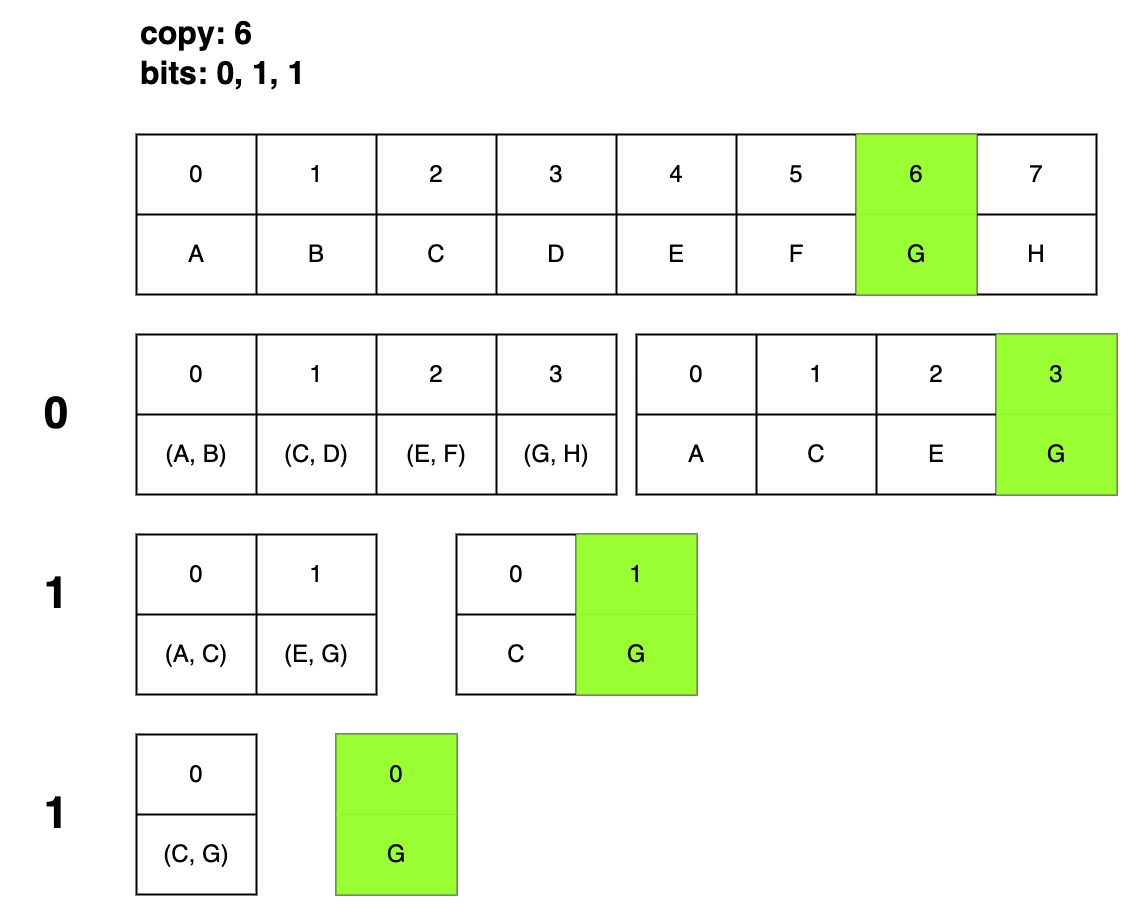
\includegraphics[width=0.8\textwidth]{gates/random_access_example.jpeg}
        \caption{Random Access Example}
        \label{fig:random-access-example}
    \end{figure}
    \begin{lstlisting}
for b in bits {
    list_items = list_items
        .iter()
        .tuples()
        .map(|(&x, &y)| builder.select_ext_generalized(b, y, x))
        .collect()
}
// Check that the one remaining element after the folding is the claimed element.
debug_assert_eq!(list_items.len(), 1);
constraints.push(builder.sub_extension(list_items[0], claimed_element));
    \end{lstlisting}
\end{itemize}

Finally, the constant is constrained -- A total of num\_extra\_constraints constraints.

In summary, there're $num\_copies*(bits + 2) + num\_extra\_constants$ constraints. Degree is $bits + 1$ which happens when repeatedly folding the list. 

\subsection{reducing}

ReducingGate is used for computes $output = old\_acc + \sum C_i*\alpha^i$ in base field.

Trace structure for this gate is like:

\begin{figure}[!ht]
    \centering
    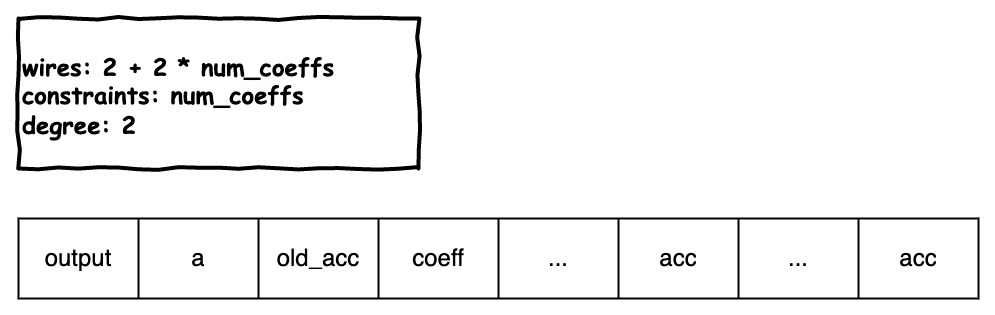
\includegraphics[width=0.8\textwidth]{gates/reducing.jpeg}
    \caption{ReducingGate}
    \label{fig:reducing}
\end{figure}

The constraint flow is relatively intuitive, initializing acc to old\_acc, then cumulative computation of polynomials by coeff in turn, 
and constraining the intermediate results of each step with acc.

\begin{lstlisting}
for i in 0..self.num_coeffs {
    let coeff = builder.convert_to_ext_algebra(coeffs[i]);
    let mut tmp = builder.mul_add_ext_algebra(acc, alpha, coeff);
    tmp = builder.sub_ext_algebra(tmp, accs[i]);
    constraints.push(tmp);
    acc = accs[i];
}
\end{lstlisting}

The number of constraints is equal to the number of coefficients. Polynomial degree is 2 which happens when calculating $coeff_i * \alpha$, sum up does not increase degree.

ReducingExtensionGate is like ReducingGate, just computations happen in extension field, constrain logic is all the same.
\subsubsection{high\_degree\_interpolation}

InterpolationGate is used for interpolation a polynomial, whose points are a (base field) coset of the multiplicative subgroup 
with the given size, and whose values are extension field elements. As for HighDegreeInterpolationGate,  allows constraints of variable degree, 
up to $1<<subgroup\_bits$. The higher degree is a tradeoff for less gates(than LowDegreeInterpolationGate).


HighDegreeInterpolationGate trace is shown in figure \ref{fig:high-degree-interpolation}

\begin{figure}[!ht]
    \centering
    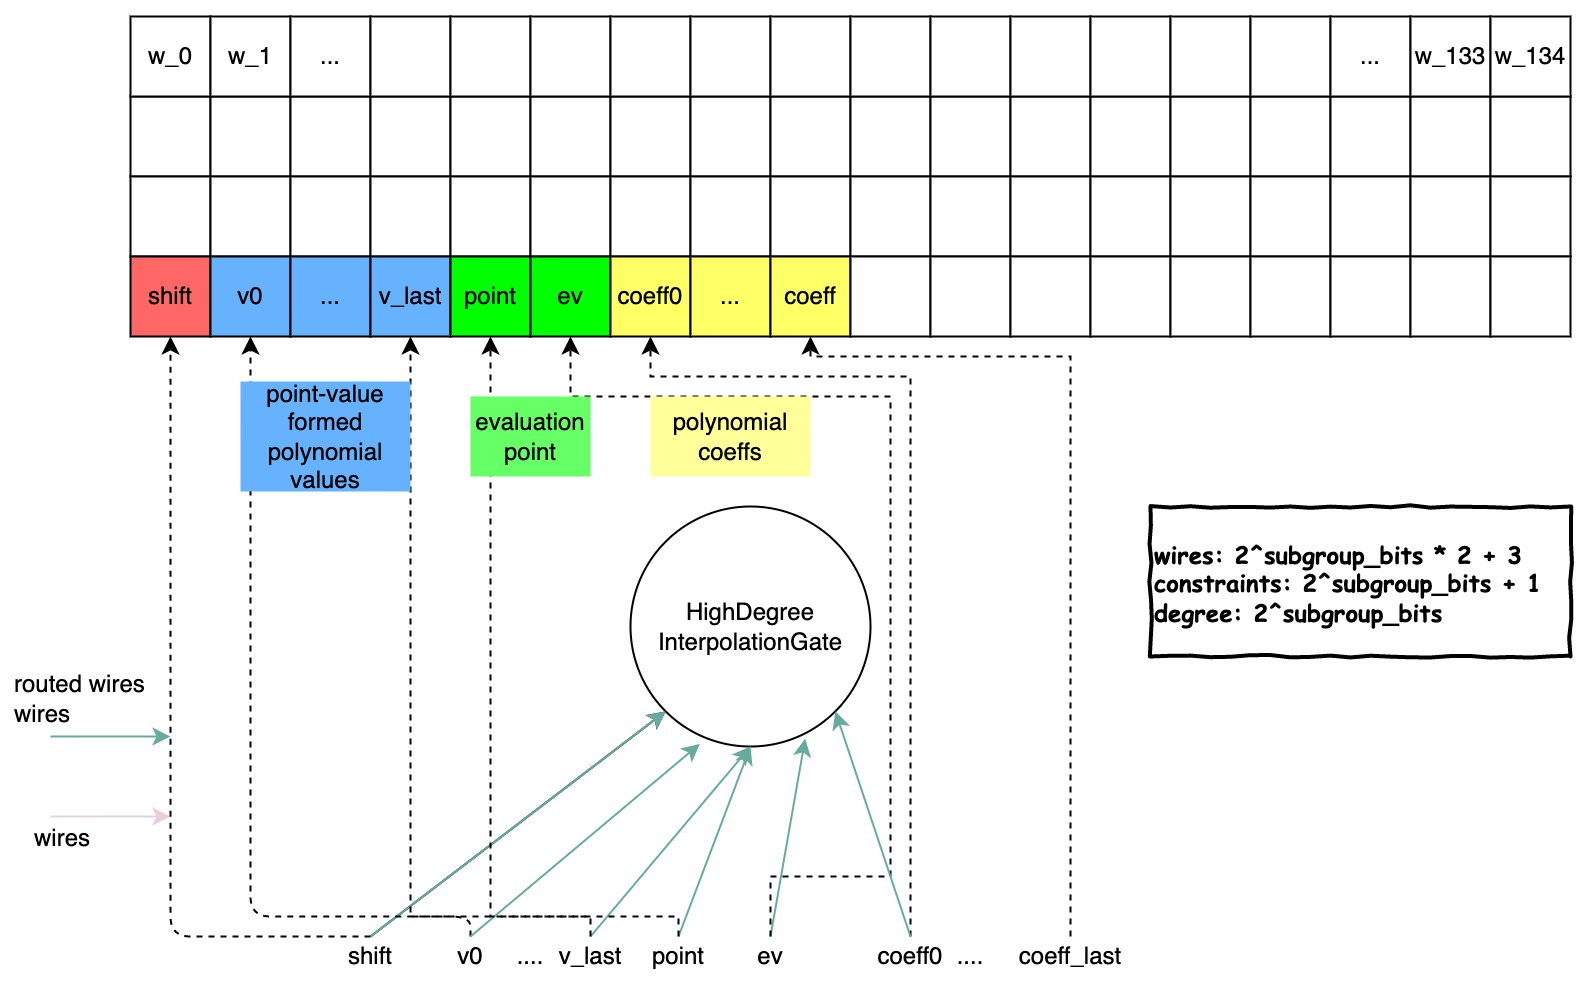
\includegraphics[width=0.8\textwidth]{gates/high_degree_interpolation.jpeg}
    \caption{HighDegreeInterpolationGate}
    \label{fig:high-degree-interpolation}
\end{figure}


Constraints:
\begin{itemize}
    \item Bring each point(from the point-value pairs) into the coefficient polynomial to compute the computed\_value, 
    and compare the constraint with the value(from the point-value pairs). -- A total of $2^{subgroup\_bits}$ constraints.
    \begin{lstlisting}
for (i, point) in coset.into_iter().enumerate() {
    let value = vars.get_local_ext_algebra(self.wires_value(i));
    let computed_value = interpolant.eval_base(point);
    constraints.extend((value - computed_value).to_basefield_array());
}
    \end{lstlisting}
    coset: $[sg, sg^2,...,sg^{2^{subgroup\_bits}}], s=shift$
    \item Evaluate the coefficient-form polynomial at evaluation point, and constrain with ev. -- 1 constraint.
\end{itemize}

The degree of this gate equals the number of points(num\_points): max point power is $num\_points - 1$, and multiplication by coefficient adds 1 degree.

Number of constraints equals $num\_points + 1$: num\_points for consistency between the coefficients and the point-value pairs, 1 constraints for the evaluation value. 
\subsubsection{low\_degree\_interpolation}

InterpolationGate is used for interpolation a polynomial, whose points are a (base field) coset of the multiplicative subgroup 
with the given size, and whose values are extension field elements. As for LowDegreeInterpolationGate,  all constraints are degree <= 2, 
low degree is a tradeoff for more gates(than HighDegreeInterpolationGate).

LowDegreeInterpolationGate trace is shown in figure \ref{fig:low-degree-interpolation}

\begin{figure}[!ht]
    \centering
    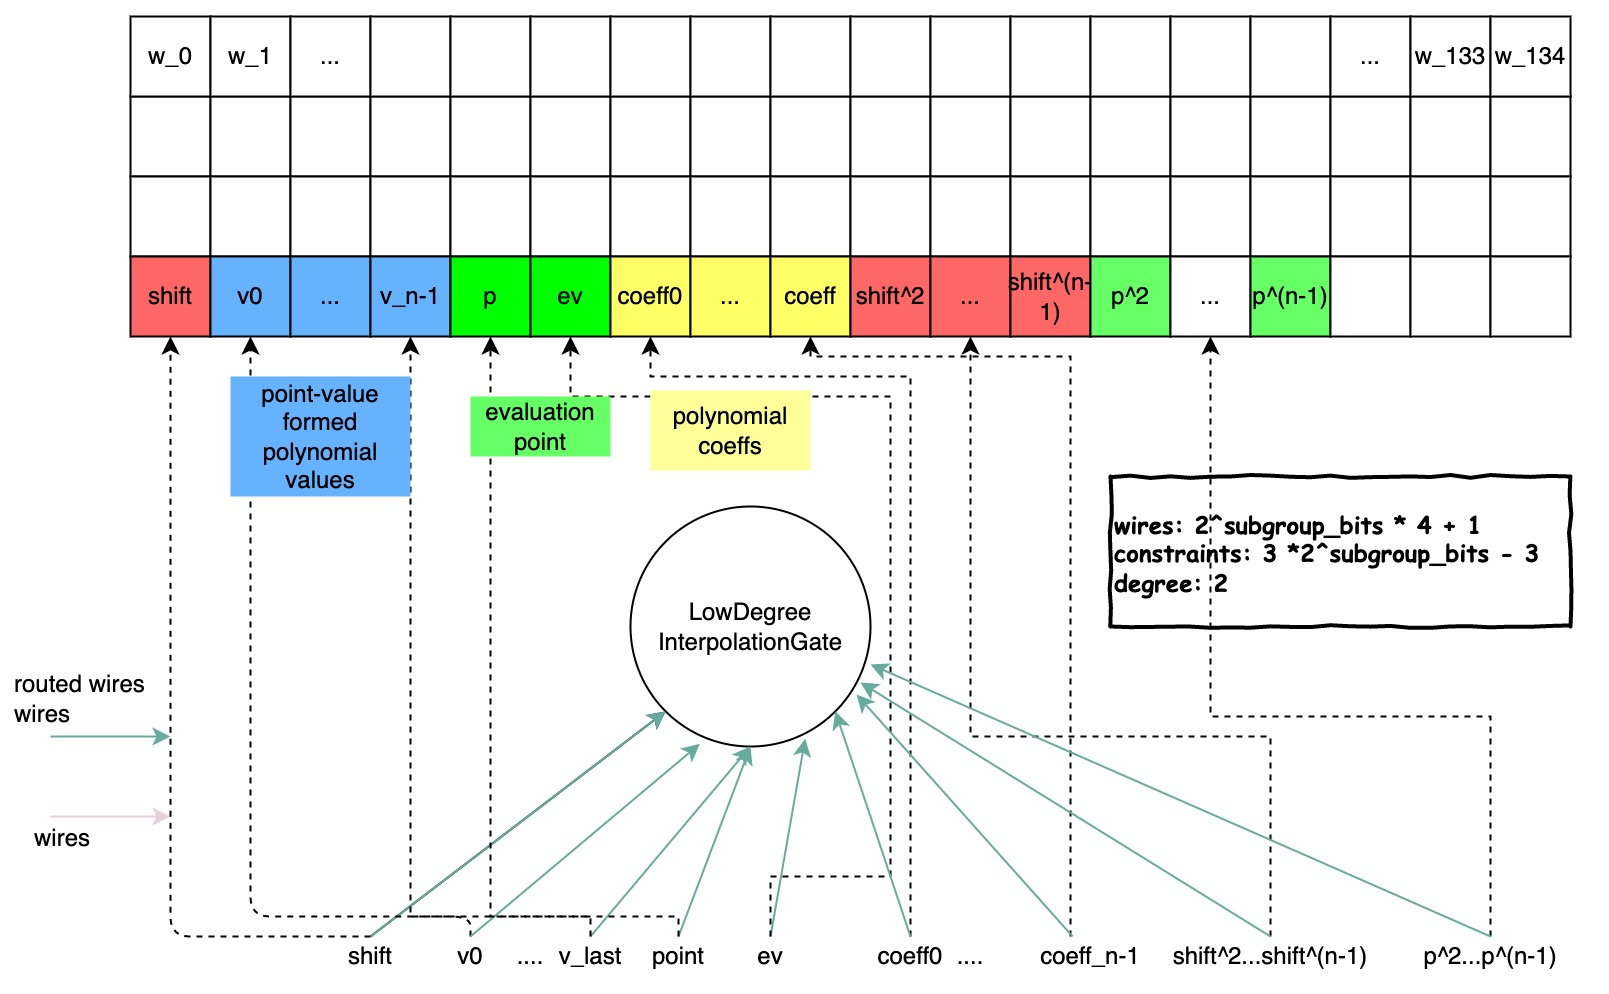
\includegraphics[width=0.8\textwidth]{gates/low_degree_interpolation.jpeg}
    \caption{LowDegreeInterpolationGate}
    \label{fig:low-degree-interpolation}
\end{figure}

Constraints:
\begin{itemize}
    \item Constrain powers of shift, from $shift^2$ to $shift^{n-1}$, a total of $2^{subgroup\_bits}-2$ constraints.
    \begin{lstlisting}
for i in 1..self.num_points() - 1 {
    constraints.push(powers_shift[i - 1] * shift - powers_shift[i]);
}
    \end{lstlisting}
    \item Bring each point(from the point-value pairs) into the coefficient polynomial to compute the computed\_value, 
    and compare the constraint with the value(from the point-value pairs). -- A total of $2^{subgroup\_bits}$ constraints.
    \item Constrain powers of evalation point. -- A total of $2^{subgroup\_bits}-2$ constraints.
    \item Evaluate the coefficient-form polynomial at evaluation point, and constrain with ev. -- 1 constraint.
\end{itemize}

As can be seen from the above constraint description, number of constraints is $3*2^{subgroup\_bits}-3$, degree of LowDegreeInterpolationGate is 2.
\subsection{U32 gates}
\subsubsection{add\_many\_u32}

U32AddManyGate is a gate to perform addition on num\_addends different 32-bit values, plus a small carry. 
There can be up to 16 operations per gate.

Gate structure is like \figref{fig:add-many-u32}.

\begin{figure}[!ht]
    \centering
    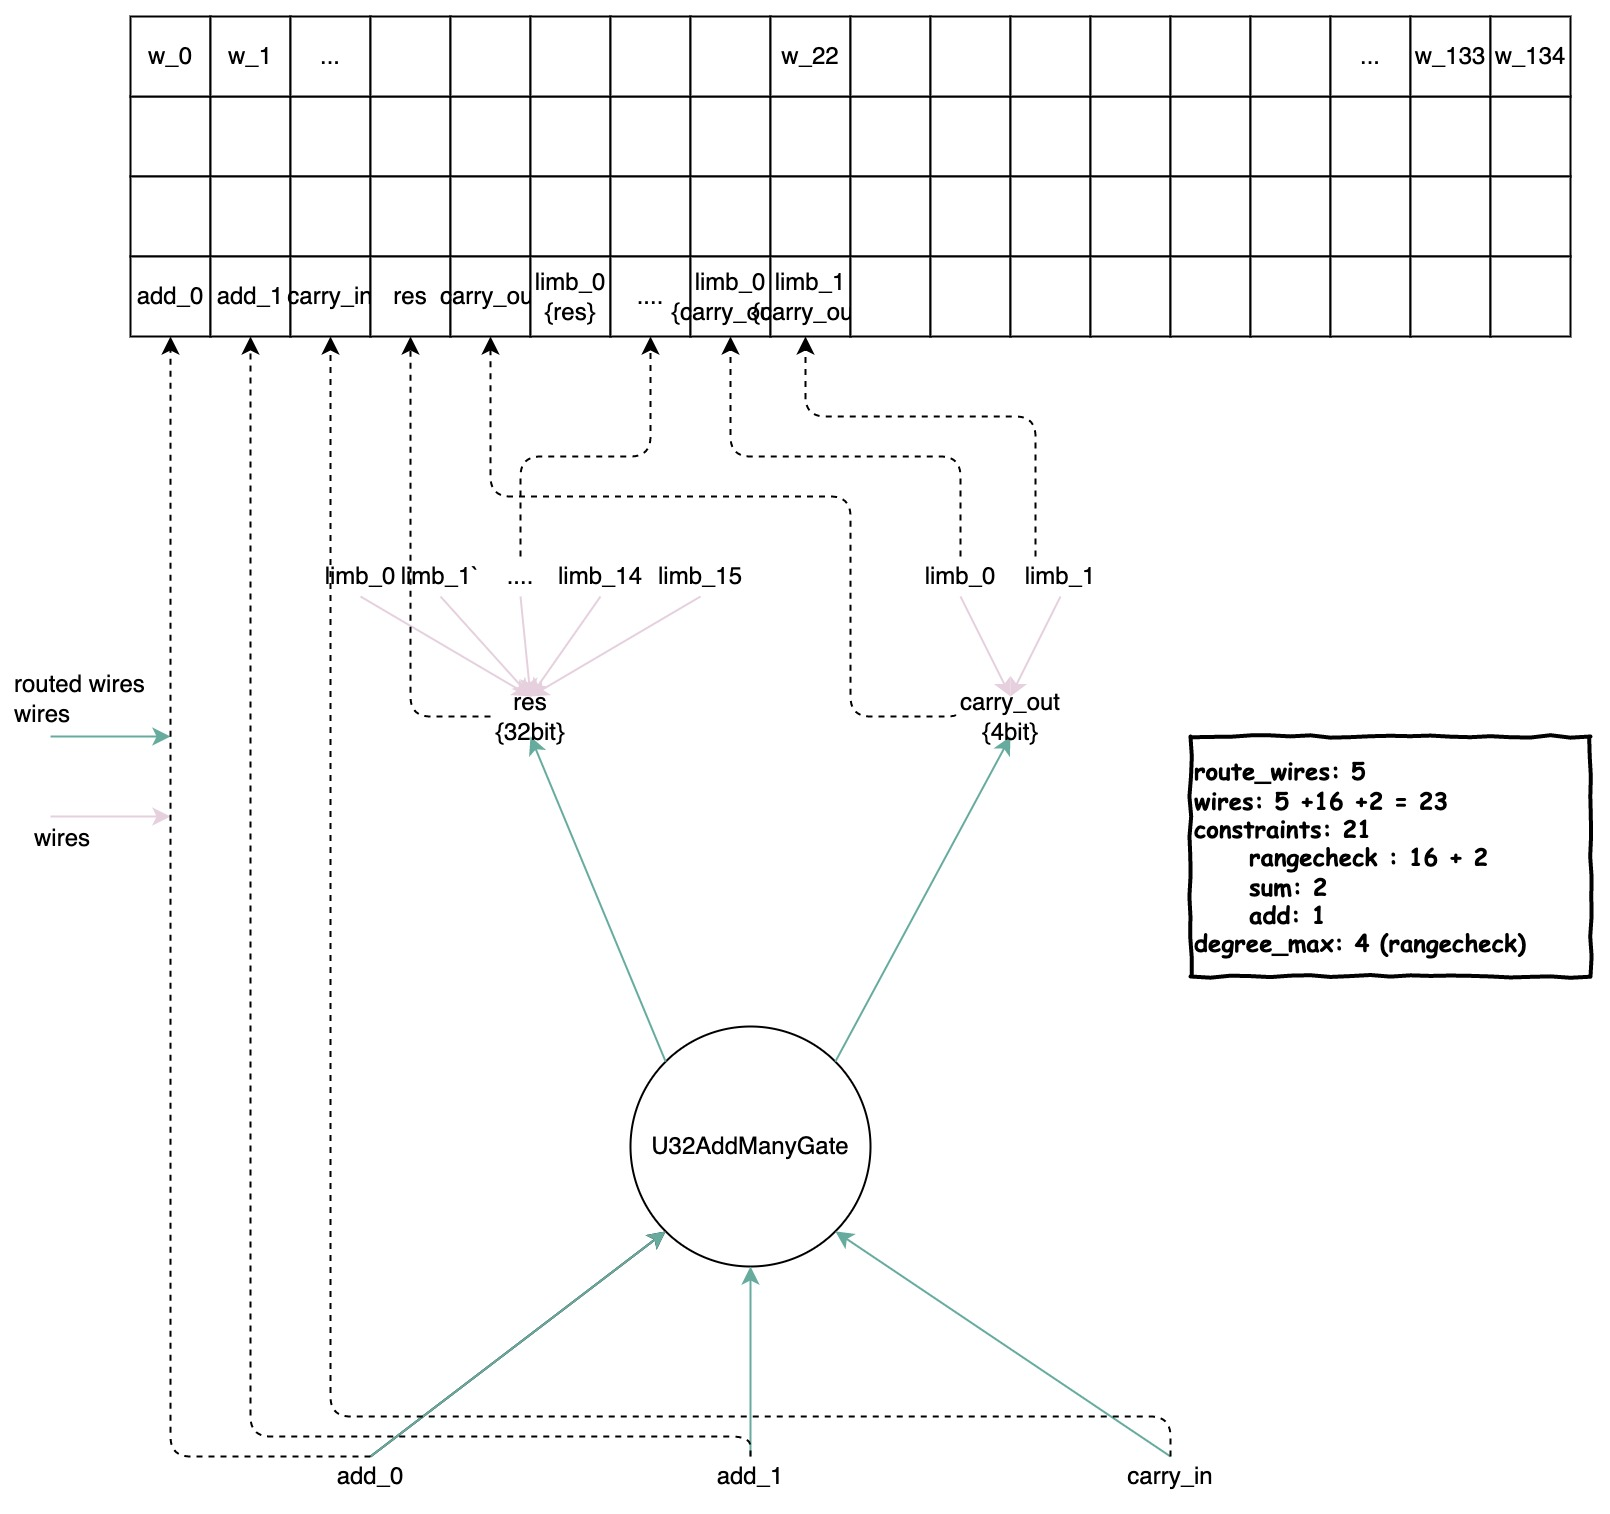
\includegraphics[width=0.8\textwidth]{gates/add_many_u32.jpeg}
    \caption{U32AddManyGate}
    \label{fig:add-many-u32}
\end{figure}

Constraints for each operation:
\begin{itemize}
    \item Constrain the result of addends summation equals results of res and carry\_out calculation. -- 1 constraint with degree 1
    \begin{lstlisting}[language=rust]
let base = F::Extension::from_canonical_u64(1 << 32u64);
let combined_output = output_carry * base + output_result;
constraints.push(combined_output - computed_output);
    \end{lstlisting}
    \item Limbs range check. -- 18(limbs) constraints with degree 4.(limbs are all 2-bits)
    \begin{lstlisting}[language=rust]
let product = (0..max_limb)
    .map(|x| this_limb - F::Extension::from_canonical_usize(x))
    .product();
constraints.push(product);
    \end{lstlisting}
    \item Constrain limbs for res and carry\_out. -- 2 constraints with degree 1.
\end{itemize}

In summary, there are 21 constraints for each operation. Degree of the gate is 4 which is needed by 4-bits limbs range check.

\subsubsection{arithmetic\_u32}

U32ArithmeticGate gate is used for compute $\text{res} = \text{mul\_0} \times \text{mul\_1} + \text{add}$. Res is store in res\_lo and res\_hi each of which can be represented by 15 limbs.

Gate structure is like \figref{fig:arithmetic-u32}.

\begin{figure}[!ht]
    \centering
    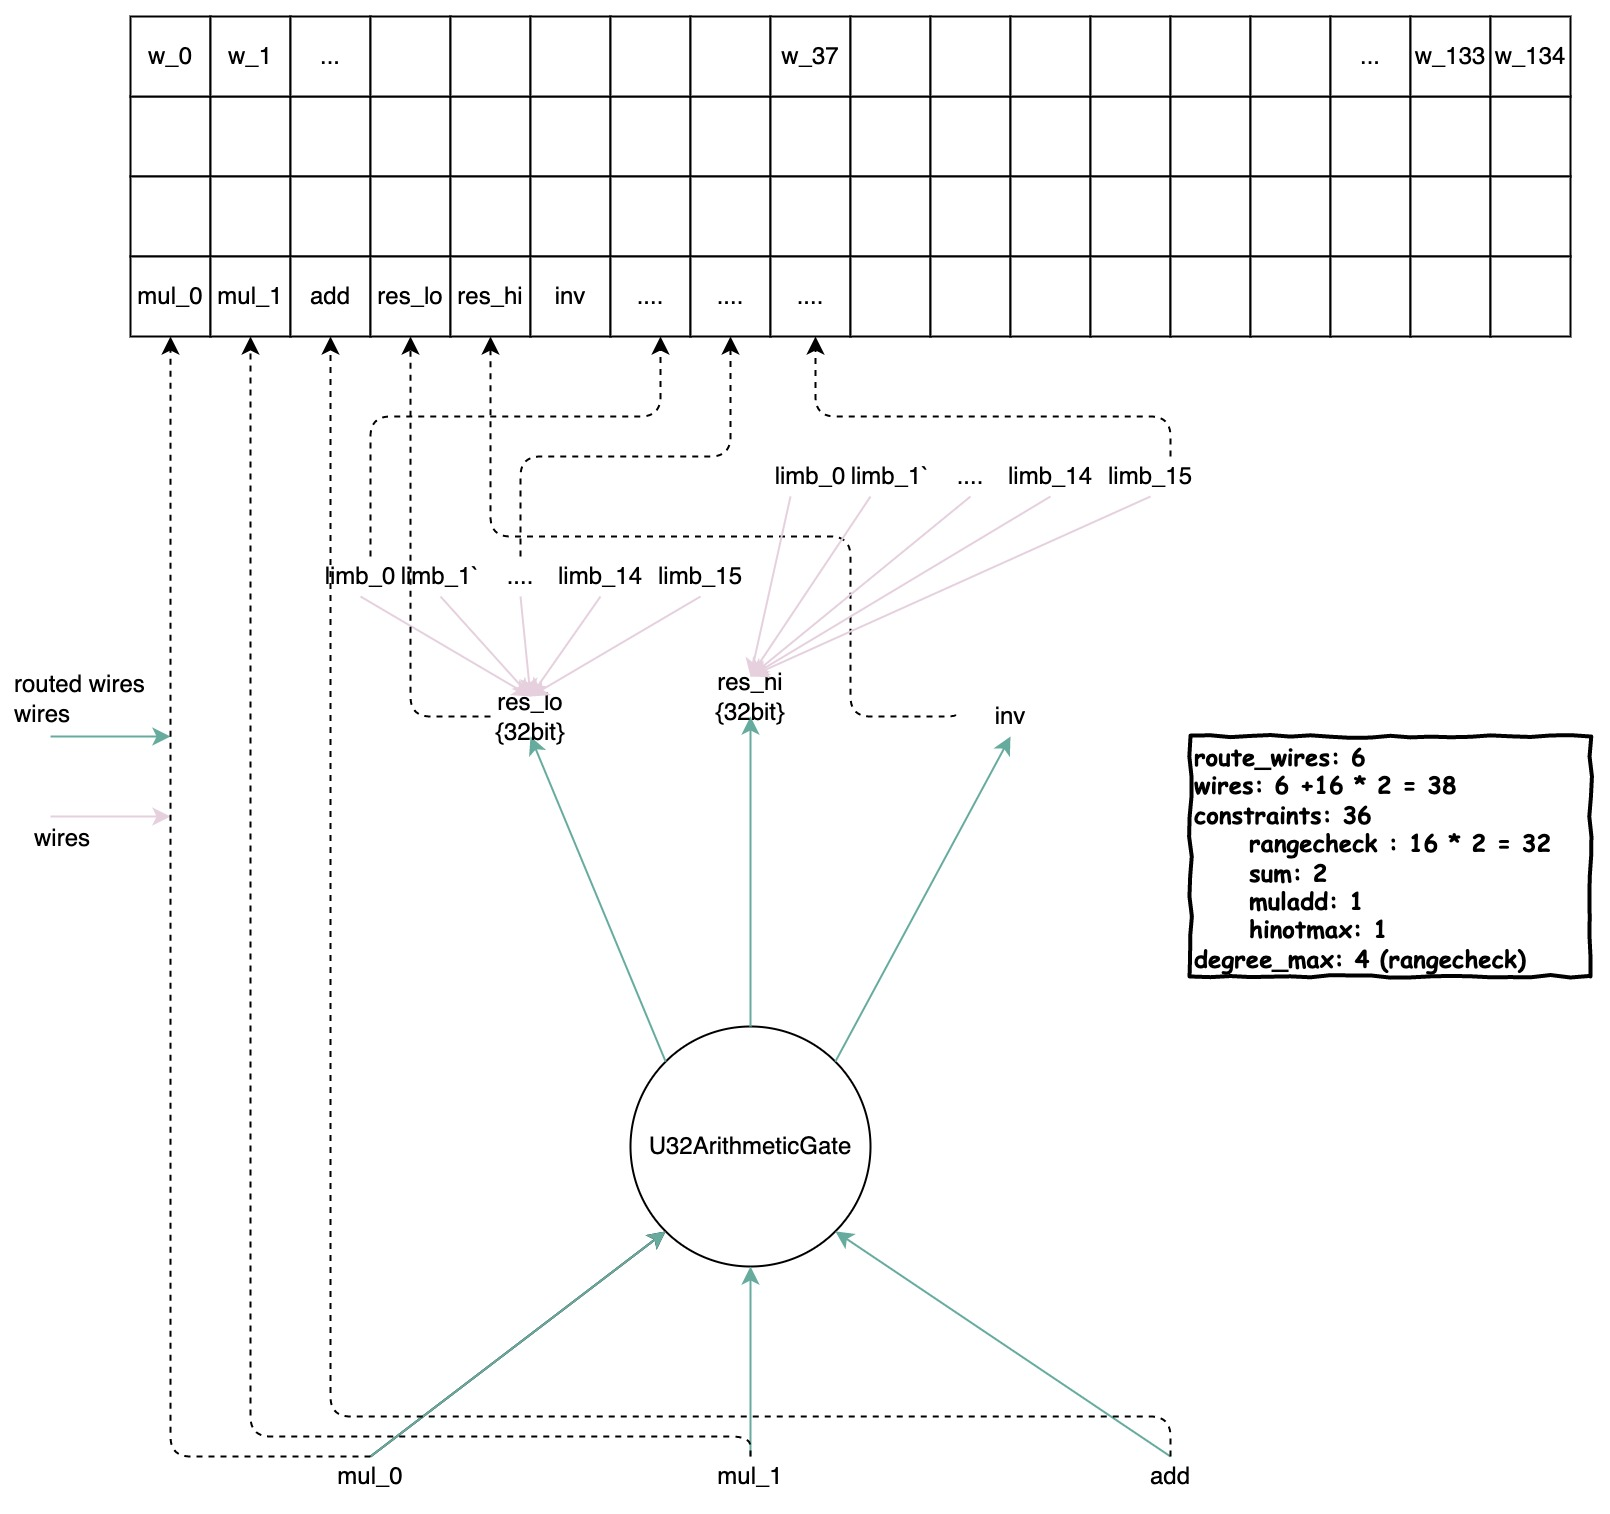
\includegraphics[width=0.8\textwidth]{gates/arithmetic_u32.jpeg}
    \caption{U32ArithmeticGate}
    \label{fig:arithmetic-u32}
\end{figure}

Constraints for each operation:
\begin{itemize}
    \item Constrain res is not overflow (less equal than \verb|max_u32 * max_u32 + max_u32|). -- 1 constraint with degree 2.
    \item Constrain combined((by res\_lo and res\_hi)) output equals computed (by \verb|mul_0 * mul_1 + add|) output. -- 1 constraint with degree 2.
    \item Limbs range check. -- 32 (limbs) constraints with degree 4. (limbs are all 2-bits)
    \item Constrain limbs for res\_lo and res\_hi. -- 2 constraints with degree 1.
\end{itemize}

In summary, there are 36 constraints for each operation. Degree of the gate is 4 which is needed by 4-bits limbs range check.
